% Embedded animations in Beamer
\documentclass[hyperref={pdfpagelabels=false}]{beamer}
\usepackage{lmodern}
% Required package
\usepackage{animate}
\usepackage{amssymb}

\usepackage[utf8]{inputenc} % this is needed for german umlauts
\usepackage[ngerman]{babel} % this is needed for german umlauts
\usepackage[T1]{fontenc}    % this is needed for correct output of umlauts in pdf

\usepackage{verbatim}
\usepackage{tikz}
\usetikzlibrary{arrows,shapes}

% see http://deic.uab.es/~iblanes/beamer_gallery/index_by_theme.html
\usetheme{Frankfurt}
\usefonttheme{professionalfonts}

\begin{document}



\setbeamercovered{transparent}
\begin{frame}{What is Dynamic Time Warping?}
    \textit{\textbf{\Large{\textcolor{blue}{Dynamic Time Warping} is }} }
    \begin{itemize}
    \onslide<1->{\item \large{An algorithm used for measuring the similarity between two temporal time series sequence }}
    \onslide<2->{\item \large{Computes the distance from the matching similar elements between two series}}
    \onslide<3->{\item \large{Used in dynamic programming to find the optimal path}}
    \end{itemize}

\end{frame}

\setbeamercovered{invisible}
\begin{frame}{Motivation for DTW}
    \textbf{\Large{Tells us basically two things :}} 
    \begin{itemize}
    \onslide<1->{\item \large{How \textcolor{blue}{similar} are two signals }}
    \onslide<2->{\item \large{Which \textcolor{blue}{points correspond to} one another}}
    \end{itemize}

\end{frame}


\setbeamercovered{transparent}

\begin{frame}{So How do you figure out how similar the Signals are?}
\begin{block}{First Approach}
    \textcolor{blue}{\textbf{Euclidean Matching :}}\\
    Compare the \textcolor{blue}{Signals} point by point\\ \\
    \onslide<2->\textit{In fact, this approach is called the "Naive Approach"}
\end{block}    
\end{frame}

\begin{frame}{So How do you figure out how similar the Signals are?}
\begin{block}{Second Approach}
    \textcolor{blue}{\textbf{Dynamic Time Warping :}}\\
    Used for two \textcolor{blue}{variable-length arrays or time sequences} to create the best possible alignment. \\ \\ 
    \onslide<2->\textit{Exploiting the temporal distortions between them.}
\end{block}    
\end{frame}

\pgfdeclarelayer{background}
\pgfdeclarelayer{foreground}
\pgfsetlayers{background,main,foreground}


% \begin{frame}{GIFs in Beamer}
% \centering
% \animategraphics[loop,width=8cm]{10}{Chandler-}{0}{44}
% \end{frame}

\begin{frame}{Similarity Detection}
\centering
\animategraphics[width=8cm]{50}{Two_repeti-}{0}{154}
\end{frame}


\begin{frame}{Euclidean Matching Vs Dynamic Time Warping}
\begin{figure}
    \begin{tikzpicture}[]
        % Draw the vertices.
        \node (1) [red] at (-4,1) {\textbullet};
        \node (2) [red] at (-3,1) {\textbullet};
        \node (3) [red] at (-2,2) {\textbullet};
        \node (4) [red] at (-1,2) {\textbullet};
        \node (5) [red] at (0,1) {\textbullet};
        \node (6) [red] at (1,1) {\textbullet};
        \node (7) [red] at (2,0) {\textbullet};
        \node (8) [red] at (3,1) {\textbullet};
        \node (9) [red] at (4,1) {\textbullet};
        \node (10) [red] at (5,1) {\textbullet};
        \node (11) [red] at (6,1) {\textbullet};


        \node (12) [blue] at (-4,-2) {\textbullet};
        \node (13) [blue] at (-3,-2) {\textbullet};
        \node (14) [blue] at (-2,-2) {\textbullet};
        \node (15) [blue] at (-1,-2) {\textbullet};
        \node (16) [blue] at (0,-1) {\textbullet};
        \node (17) [blue] at (1,-1) {\textbullet};
        \node (18) [blue] at (2,-2) {\textbullet};
        \node (19) [blue] at (3,-2) {\textbullet};
        \node (20) [blue] at (4,-2) {\textbullet};
        \node (21) [blue] at (5,-3) {\textbullet};
        \node (22) [blue] at (6,-2.5) {\textbullet};
        \node (23) [blue] at (7,-2) {\textbullet};

        % Connect vertices with edges and draw weights
        \draw[line width=0.25mm, red] (-4,1)--(-3,1);
        \draw[line width=0.25mm,red] (-3,1)--(-2,2);
        \draw[line width=0.25mm,red] (-2,2)--(-1,2);
        \draw[line width=0.25mm,red] (-1,2)--(0,1);
        \draw[line width=0.25mm,red] (0,1)--(1,1);
        \draw[line width=0.25mm,red] (1,1)--(2,0);
        \draw[line width=0.25mm,red] (2,0)--(3,1);
        \draw[line width=0.25mm,red] (3,1)--(4,1);
        \draw[line width=0.25mm,red] (4,1)--(5,1);
        \draw[line width=0.25mm,red] (5,1)--(6,1);


        \draw[line width=0.25mm, blue] (-4,-2)--(-3,-2);
        \draw[line width=0.25mm,blue] (-3,-2)--(-2,-2);
        \draw[line width=0.25mm,blue] (-2,-2)--(-1,-2);
        \draw[line width=0.25mm,blue] (-1,-2)--(0,-1);
        \draw[line width=0.25mm,blue] (0,-1)--(1,-1);
        \draw[line width=0.25mm,blue] (1,-1)--(2,-2);
        \draw[line width=0.25mm,blue] (2,-2)--(3,-2);
        \draw[line width=0.25mm,blue] (3,-2)--(4,-2);
        \draw[line width=0.25mm,blue] (4,-2)--(5,-3);
        \draw[line width=0.25mm,blue] (5,-3)--(6,-2.5);
        \draw[line width=0.25mm,blue] (6,-2.5)--(7,-2);
        
        % \path [red] (1) edge node {} (2);
     

        \begin{pgfonlayer}{background}
            \path<2-5>[draw,line width=0.5mm,-,black!50] (1.center) edge node {} (12.center);
            \path<3-5>[draw,line width=0.5mm,-,black!50] (2.center) edge node {} (13.center);
            \path<5-5>[draw,line width=0.5mm,-,black!50] (3.center) edge node {} (14.center);
            \path<5-5>[draw,line width=0.5mm,-,black!50] (4.center) edge node {} (15.center);
            \path<5-5>[draw,line width=0.5mm,-,black!50] (5.center) edge node {} (16.center);
            \path<5-5>[draw,line width=0.5mm,-,black!50] (6.center) edge node {} (17.center);
            \path<5-5>[draw,line width=0.5mm,-,black!50] (7.center) edge node {} (18.center);
            \path<5-5>[draw,line width=0.5mm,-,black!50] (8.center) edge node {} (19.center);
            \path<5-5>[draw,line width=0.5mm,-,black!50] (9.center) edge node {} (20.center);
            \path<5-5>[draw,line width=0.5mm,-,black!50] (10.center) edge node {} (21.center);
            \path<5-5>[draw,line width=0.5mm,-,black!50] (11.center) edge node {} (22.center);
            % \path<10->[draw,line width=5pt,-,red!50] (b.center) edge node {} (d.center);
            % \path<12->[draw,line width=5pt,-,red!50] (d.center) edge node {} (e.center);

            \node<4-5> (x1) [above of = 1, yshift = -0.5cm] {$x_1$};
            \node<4-5> (x2) [above of = 2, yshift = -0.5cm] {$x_2$};
            \node<4-5> (y1) [below of = 12, yshift = 0.5cm] {$y_1$};
            \node<4-5> (y2) [below of = 13, yshift = 0.5cm] {$y_2$};

            \node<5-5> (xn) [above of = 11, yshift = -0.5cm] {$x_n$};
            \node<5-5> (yn) [below of = 22, yshift = 0.5cm] {$y_n$};
            

            % \path<6-6>[draw,line width=0.5mm,-,black!50] (1.center) edge node {} (12.center);
            % \path<6-6>[draw,line width=0.5mm,-,black!50] (1.center) edge node {} (13.center);
            % \path<6-6>[draw,line width=0.5mm,-,black!50] (1.center) edge node {} (14.center);
            % \path<6-6>[draw,line width=0.5mm,-,black!50] (2.center) edge node {} (15.center);
            % \path<6-6>[draw,line width=0.5mm,-,black!50] (3.center) edge node {} (16.center);
            % \path<6-6>[draw,line width=0.5mm,-,black!50] (4.center) edge node {} (17.center);
            % \path<6-6>[draw,line width=0.5mm,-,black!50] (5.center) edge node {} (18.center);
            % \path<6-6>[draw,line width=0.5mm,-,black!50] (6.center) edge node {} (19.center);
            % \path<6-6>[draw,line width=0.5mm,-,black!50] (7.center) edge node {} (20.center);
            % \path<6-6>[draw,line width=0.5mm,-,black!50] (8.center) edge node {} (21.center);
            % \path<6-6>[draw,line width=0.5mm,-,black!50] (9.center) edge node {} (22.center);
            % \path<6-6>[draw,line width=0.5mm,-,black!50] (10.center) edge node {} (22.center);
            % \path<6-6>[draw,line width=0.5mm,-,black!50] (11.center) edge node {} (23.center);

        \end{pgfonlayer}
    \end{tikzpicture}
   
\end{figure}
\end{frame}

\begin{frame}{Euclidean Matching Vs Dynamic Time Warping}
\begin{figure}
    \begin{tikzpicture}[]
        % Draw the vertices.
        \node (1) [red] at (-4,1) {\textbullet};
        \node (2) [red] at (-3,1) {\textbullet};
        \node (3) [red] at (-2,2) {\textbullet};
        \node (4) [red] at (-1,2) {\textbullet};
        \node (5) [red] at (0,1) {\textbullet};
        \node (6) [red] at (1,1) {\textbullet};
        \node (7) [red] at (2,0) {\textbullet};
        \node (8) [red] at (3,1) {\textbullet};
        \node (9) [red] at (4,1) {\textbullet};
        \node (10) [red] at (5,1) {\textbullet};
        \node (11) [red] at (6,1) {\textbullet};


        \node (12) [blue] at (-4,-2) {\textbullet};
        \node (13) [blue] at (-3,-2) {\textbullet};
        \node (14) [blue] at (-2,-2) {\textbullet};
        \node (15) [blue] at (-1,-2) {\textbullet};
        \node (16) [blue] at (0,-1) {\textbullet};
        \node (17) [blue] at (1,-1) {\textbullet};
        \node (18) [blue] at (2,-2) {\textbullet};
        \node (19) [blue] at (3,-2) {\textbullet};
        \node (20) [blue] at (4,-2) {\textbullet};
        \node (21) [blue] at (5,-3) {\textbullet};
        \node (22) [blue] at (6,-2.5) {\textbullet};
        \node (23) [blue] at (7,-2) {\textbullet};

        % Connect vertices with edges and draw weights
        \draw[line width=0.25mm, red] (-4,1)--(-3,1);
        \draw[line width=0.25mm,red] (-3,1)--(-2,2);
        \draw[line width=0.25mm,red] (-2,2)--(-1,2);
        \draw[line width=0.25mm,red] (-1,2)--(0,1);
        \draw[line width=0.25mm,red] (0,1)--(1,1);
        \draw[line width=0.25mm,red] (1,1)--(2,0);
        \draw[line width=0.25mm,red] (2,0)--(3,1);
        \draw[line width=0.25mm,red] (3,1)--(4,1);
        \draw[line width=0.25mm,red] (4,1)--(5,1);
        \draw[line width=0.25mm,red] (5,1)--(6,1);


        \draw[line width=0.25mm, blue] (-4,-2)--(-3,-2);
        \draw[line width=0.25mm,blue] (-3,-2)--(-2,-2);
        \draw[line width=0.25mm,blue] (-2,-2)--(-1,-2);
        \draw[line width=0.25mm,blue] (-1,-2)--(0,-1);
        \draw[line width=0.25mm,blue] (0,-1)--(1,-1);
        \draw[line width=0.25mm,blue] (1,-1)--(2,-2);
        \draw[line width=0.25mm,blue] (2,-2)--(3,-2);
        \draw[line width=0.25mm,blue] (3,-2)--(4,-2);
        \draw[line width=0.25mm,blue] (4,-2)--(5,-3);
        \draw[line width=0.25mm,blue] (5,-3)--(6,-2.5);
        \draw[line width=0.25mm,blue] (6,-2.5)--(7,-2);
        
        % \path [red] (1) edge node {} (2);
     

        \begin{pgfonlayer}{background}
            \path<1-1>[draw,line width=0.5mm,-,black!50] (1.center) edge node {} (12.center);
            \path<1-1>[draw,line width=0.5mm,-,black!50] (2.center) edge node {} (13.center);
            \path<1-1>[draw,line width=0.5mm,-,black!50] (3.center) edge node {} (14.center);
            \path<1-1>[draw,line width=0.5mm,-,black!50] (4.center) edge node {} (15.center);
            \path<1-1>[draw,line width=0.5mm,-,black!50] (5.center) edge node {} (16.center);
            \path<1-1>[draw,line width=0.5mm,-,black!50] (6.center) edge node {} (17.center);
            \path<1-1>[draw,line width=0.5mm,-,black!50] (7.center) edge node {} (18.center);
            \path<1-1>[draw,line width=0.5mm,-,black!50] (8.center) edge node {} (19.center);
            \path<1-1>[draw,line width=0.5mm,-,black!50] (9.center) edge node {} (20.center);
            \path<1-1>[draw,line width=0.5mm,-,black!50] (10.center) edge node {} (21.center);
            \path<1-1>[draw,line width=0.5mm,-,black!50] (11.center) edge node {} (22.center);
            % \path<10->[draw,line width=5pt,-,red!50] (b.center) edge node {} (d.center);
            % \path<12->[draw,line width=5pt,-,red!50] (d.center) edge node {} (e.center);

            \node<1-1> (x1) [above of = 1, yshift = -0.5cm] {$x_1$};
            \node<1-1> (x2) [above of = 2, yshift = -0.5cm] {$x_2$};
            \node<1-1> (y1) [below of = 12, yshift = 0.5cm] {$y_1$};
            \node<1-1> (y2) [below of = 13, yshift = 0.5cm] {$y_2$};

            \node<1-1> (xn) [above of = 11, yshift = -0.5cm] {$x_n$};
            \node<1-1> (yn) [below of = 22, yshift = 0.5cm] {$y_n$};
            

        \end{pgfonlayer}
    \end{tikzpicture}
   
\end{figure}

Formula can be written as :
\begin{equation}    
     d(x_1_:_N,y_1_:_M) = \sum_{i=1}^n |x_i-y_i|
\end{equation}

\end{frame}

\begin{frame}{Euclidean Matching Vs Dynamic Time Warping}
\begin{figure}
    \begin{tikzpicture}[]
        % Draw the vertices.
        \node (1) [red] at (-4,1) {\textbullet};
        \node (2) [red] at (-3,1) {\textbullet};
        \node (3) [red] at (-2,2) {\textbullet};
        \node (4) [red] at (-1,2) {\textbullet};
        \node (5) [red] at (0,1) {\textbullet};
        \node (6) [red] at (1,1) {\textbullet};
        \node (7) [red] at (2,0) {\textbullet};
        \node (8) [red] at (3,1) {\textbullet};
        \node (9) [red] at (4,1) {\textbullet};
        \node (10) [red] at (5,1) {\textbullet};
        \node (11) [red] at (6,1) {\textbullet};


        \node (12) [blue] at (-4,-2) {\textbullet};
        \node (13) [blue] at (-3,-2) {\textbullet};
        \node (14) [blue] at (-2,-2) {\textbullet};
        \node (15) [blue] at (-1,-2) {\textbullet};
        \node (16) [blue] at (0,-1) {\textbullet};
        \node (17) [blue] at (1,-1) {\textbullet};
        \node (18) [blue] at (2,-2) {\textbullet};
        \node (19) [blue] at (3,-2) {\textbullet};
        \node (20) [blue] at (4,-2) {\textbullet};
        \node (21) [blue] at (5,-3) {\textbullet};
        \node (22) [blue] at (6,-2.5) {\textbullet};
        \node (23) [blue] at (7,-2) {\textbullet};

        % Connect vertices with edges and draw weights
        \draw[line width=0.25mm, red] (-4,1)--(-3,1);
        \draw[line width=0.25mm,red] (-3,1)--(-2,2);
        \draw[line width=0.25mm,red] (-2,2)--(-1,2);
        \draw[line width=0.25mm,red] (-1,2)--(0,1);
        \draw[line width=0.25mm,red] (0,1)--(1,1);
        \draw[line width=0.25mm,red] (1,1)--(2,0);
        \draw[line width=0.25mm,red] (2,0)--(3,1);
        \draw[line width=0.25mm,red] (3,1)--(4,1);
        \draw[line width=0.25mm,red] (4,1)--(5,1);
        \draw[line width=0.25mm,red] (5,1)--(6,1);


        \draw[line width=0.25mm, blue] (-4,-2)--(-3,-2);
        \draw[line width=0.25mm,blue] (-3,-2)--(-2,-2);
        \draw[line width=0.25mm,blue] (-2,-2)--(-1,-2);
        \draw[line width=0.25mm,blue] (-1,-2)--(0,-1);
        \draw[line width=0.25mm,blue] (0,-1)--(1,-1);
        \draw[line width=0.25mm,blue] (1,-1)--(2,-2);
        \draw[line width=0.25mm,blue] (2,-2)--(3,-2);
        \draw[line width=0.25mm,blue] (3,-2)--(4,-2);
        \draw[line width=0.25mm,blue] (4,-2)--(5,-3);
        \draw[line width=0.25mm,blue] (5,-3)--(6,-2.5);
        \draw[line width=0.25mm,blue] (6,-2.5)--(7,-2);
        
        % \path [red] (1) edge node {} (2);
     

        \begin{pgfonlayer}{background}
            

            \path<1-1>[draw,line width=0.5mm,-,black!50] (1.center) edge node {} (12.center);
            \path<1-1>[draw,line width=0.5mm,-,black!50] (1.center) edge node {} (13.center);
            \path<1-1>[draw,line width=0.5mm,-,black!50] (1.center) edge node {} (14.center);
            \path<1-1>[draw,line width=0.5mm,-,black!50] (2.center) edge node {} (15.center);
            \path<1-1>[draw,line width=0.5mm,-,black!50] (3.center) edge node {} (16.center);
            \path<1-1>[draw,line width=0.5mm,-,black!50] (4.center) edge node {} (17.center);
            \path<1-1>[draw,line width=0.5mm,-,black!50] (5.center) edge node {} (18.center);
            \path<1-1>[draw,line width=0.5mm,-,black!50] (6.center) edge node {} (19.center);
            \path<1-1>[draw,line width=0.5mm,-,black!50] (7.center) edge node {} (20.center);
            \path<1-1>[draw,line width=0.5mm,-,black!50] (8.center) edge node {} (21.center);
            \path<1-1>[draw,line width=0.5mm,-,black!50] (9.center) edge node {} (22.center);
            \path<1-1>[draw,line width=0.5mm,-,black!50] (10.center) edge node {} (22.center);
            \path<1-1>[draw,line width=0.5mm,-,black!50] (11.center) edge node {} (23.center);

        \end{pgfonlayer}
    \end{tikzpicture}
   
\end{figure}
\end{frame}

\begin{frame}{Dynamic Time Warping}
   
\begin{center}
  \begin{tabular}{|c|c|}
    \hline
    \begin{minipage}{0.3\textwidth}
      \centering
      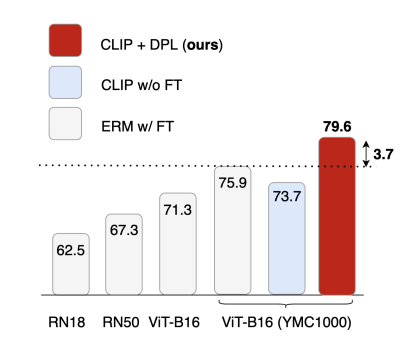
\includegraphics[width=\linewidth]{1.png}
    \end{minipage}
    &
    \begin{minipage}{0.6\textwidth}
      \centering
      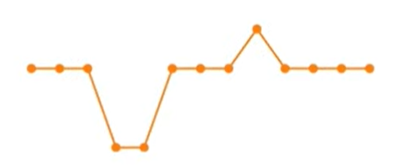
\includegraphics[width=0.3\linewidth]{2.png}
      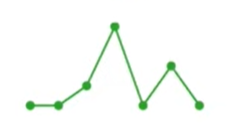
\includegraphics[width=0.3\linewidth]{3.png}
    \end{minipage}
    \\
    \hline
  \end{tabular}
\end{center}

% \begin{figure}
%     \centering
%     \begin{subfigure}{\textwidth}
%      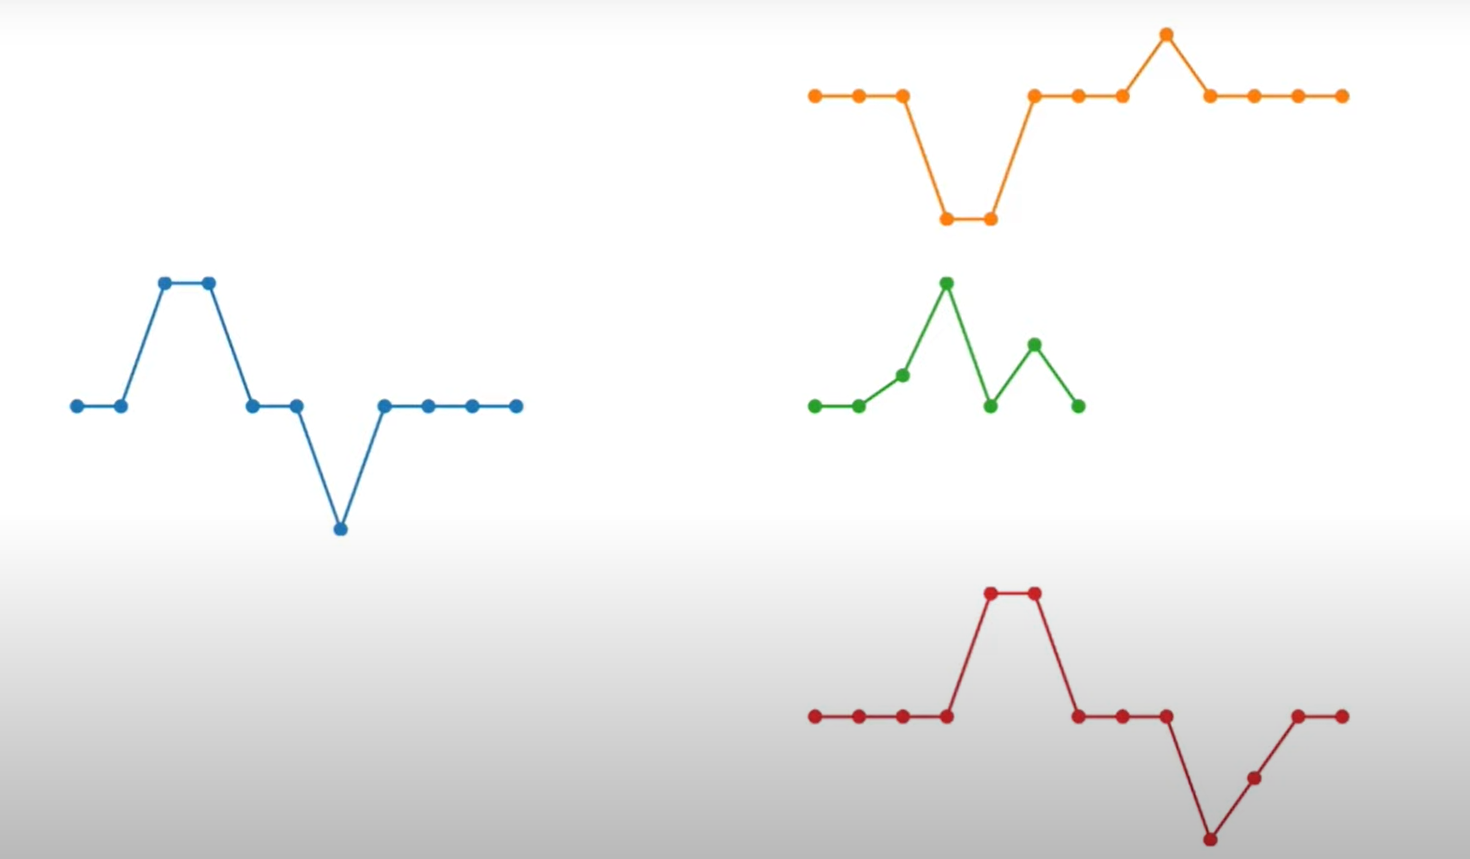
\includegraphics[width = \linewidth]{d.p}
%     \label{fig:my_label}
%     \end{subfigure}
% \end{figure}

\end{frame}


\begin{frame}{How DTW is Different?}
\begin{columns}
\column{0.5\textwidth}
\large{\textbf{Euclidean Matching}}
\begin{itemize}
    \item[$\checkmark$] One to one point Comparison 
    \item[$\checkmark$] That's why compares only time series of same length 
\end{itemize}

\column{0.5\textwidth}
\large{\textbf{Dynamic Time Warping}}
\begin{itemize}
    \item[$\checkmark$] Allows many-to-one comparisons 
    \item[$\checkmark$] Time series of different length can be compared
\end{itemize}
    
\end{columns} 
\end{frame}

\end{document}



